\documentclass[10pt]{article}
\usepackage[a4paper,left=2.54cm,top=2.54cm,right=2.54cm,bottom=2.54cm]{geometry}
\usepackage{fancyhdr}
\setlength{\headsep}{1.40cm} % Adjust the space after the header
\usepackage{afterpage}
\usepackage{setspace}
\usepackage{bibspacing}
\singlespacing

%%%% YOU CAN PUT YOUR OWN DEFINITIONS HERE
\newfont{\toto}{msbm10 at 12 pt}
\newfont{\ithd}{cmr9}
\newcommand{\equa}[1]{(\ref{eq:#1})}
\newcommand{\laeq}[1]{\label{eq:#1}}
\newcommand{\figu}[1]{\ref{fig:#1}}
\newcommand{\lafi}[1]{\label{fig:#1}}
\newcommand{\fmo}{\tilde{U}}  
\newcommand{\fve}{\tilde{u}}
\newcommand{\Dt}{\Delta t}

\newcommand{\R}{\mathbb{R}} 
\newcommand{\Z}{\mathbb{Z}}
\newcommand{\si}[1]{\rm\scriptscriptstyle{#1}}
%%%% END OF YOUR DEFINITIONS 
 
\pagestyle{fancyplain}
\renewcommand{\headrulewidth}{0pt}

\usepackage{amsmath,amsthm,amsfonts,amssymb}
\usepackage[pdftex]{graphicx} 
\usepackage[T1]{fontenc}

%%%% CONFERENCE HEADER. REPLACE xxxx WITH 4-DIGIT PAPER NUMBER ASSIGNED BY CONFERENCE COMMITTEE.

% \rhead{\ithd{\bf ICCFD12-2024-xxxx\\  \   \\}}
\lhead{\ithd{\bf Twelfth International Conference on \\      
Computational Fluid Dynamics (ICCFD12), \\
Kobe, Japan, July 14-19, 2024
}}
% Define the left and center headers to be empty or contain fixed content
\rhead{}
\chead{}

\usepackage{titling}
\setlength{\droptitle}{0em}  
\pretitle{\vspace{-4em}\begin{center}\LARGE}
\posttitle{\end{center}\vspace{-1em}}
\preauthor{\begin{center}\large}
\postauthor{\end{center}\vspace{-3em}}


\title{
\bf Paper Template of 12th International Conference on Computational Fluid Dynamics in Kobe, Japan 2024
}
\author{
D. Reynolds$^{*}$, C. Kelly$^{*}$ and F. Reynolds$^{*,**}$\\
Corresponding author: d.reynolds@paddyspub.xyz \\
$^{*}$ Paddy's Pub, USA.\\
$^{**}$ Sunny Beach Resort, USA.
}
\date{}

\begin{document}

%%%% TITLE
\maketitle
\afterpage{\fancyhead{}}

%%%% ABSTRACT AND KEYWORDS
%\vskip0.5cm
\centerline{
\begin{minipage}[t]{150mm}
{\bf Abstract:} 
The body of your abstract belongs here. ICCFD is the outcome of the merger of two important CFD conferences: the International Conference on Numerical Methods in Fluid Dynamics, ICNMFD (since 1969) and International Symposium on Computational Fluid Dynamics, ISCFD (since 1985). The first ICCFD conference was held in 2000 in Kyoto, the second in 2002 in Sydney, the third in 2004 in Toronto, the fourth in 2006 in Ghent, the fifth in 2008 in Seoul, the sixth in 2010 in St Petersburg, the seventh in Hawaii in 2012, the eighth in Chengdu in 2014, the ninth in Istanbul in 2016, the tenth in Barcelona in 2018, and the Eleventh in Hawaii in 2022. The Twelfth conference, ICCFD12 will be held on the Kobe, Japan in July 2024.
\vskip0.2cm
{\it Keywords:} Numerical Algorithms, Computational Fluid Dynamics, Turbulence Modeling, Aeroacoustics. \\
\end{minipage}
}
\vskip0.5cm

%%%% MAIN PART
\section{Introduction}
This is the main part of the paper. Its length should be no longer than {\bf 25 pages}, including key figures and references. 
It can be divided in as many sections as you decide. The paper must be prepared using this template 
and compiled using standard \LaTeX, generating a {\bf PDF file} that will be finally uploaded. If
another kind of word processor is utilized, please adhere to the formatting provided in the PDF template.


\section{Problem Statement}
This document allows you to easily include references \cite{book,journalpaper}, equations, figures (see Figure \figu{logo}) or anything else you
desire into a clean and compact environment of \LaTeX.  For example if you'd like to impress a date you can write
the unsteady heat equation as
\begin{eqnarray}
\frac{\partial \mathbf{V}}{\partial t} - \alpha \left( \frac{\partial^2 \mathbf{V}}{\partial x^2} +
       \frac{\partial^2 \mathbf{V}}{\partial y^2} +
       \frac{\partial^2 \mathbf{V}}{\partial z^2} \right)
= 0
\laeq{heat}
\end{eqnarray}
where $x, y, z$ are the space dimensions and $\alpha$ is a parameter.  If you felt inclined you could define $\mathbf{V}$ as
%
$$\mathbf{V} = y^2 z - \text{cos}(0.1 x)$$
%
for a non-exact solution.  Computational fluid dynamics~\cite{paper} can be used to discretize the equations, apply boundary conditions and 
simulation the unsteady nature of the flow.  An innovative method to simulate the heat equation could even be submitted to ICCFD12.

  The scope of ICCFD12~\cite{web} is devoted to all innovative aspects of CFD, basic and applied.  Subjects of interest include but are not limited
to: 
\begin{itemize}

    \item Innovative algorithm development for flow simulations: higher-order methods, iterative methods, parallel
          algorithms, mesh adaptation, grid generation, meshless methods, immersed boundary methods and level-set
          methods. 
          
    \item Advances in modeling of flow physics in the area of: steady and unsteady flows, compressible and incompressible 
          flows, flows in porous media, hypersonic and reacting flows, turbulence (transition, DNS/LES, etc.), multi-phase 
          flows, boundary layer stability and vortex dynamics. 
          
    \item Advanced multidisciplinary applications using the above mentioned technologies: aeroacoustics, flow
          control, biomedical fluid mechanics, large scale applications, verification and validation methods, and
          turbomachinery. 
          
\end{itemize}

\begin{figure}[t]
  \centering 
  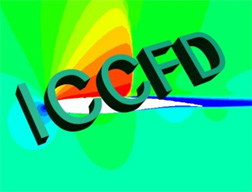
\includegraphics[height=2.0in]{exampleFigure.jpg}
  \caption{This is the logo of ICCFD.}
  \lafi{logo}
\end{figure}


\subsection{Subsection Title Example}


\subsubsection{Sub-subsection Title Example}


\section{Conclusion and Future Work}
ICCFD12 will be held at the Kobe international conference center in Port Island, Kobe, Japan. We look forward to welcoming you all to what we hope will be a memorable event.


%%%% BIBLIOGRAPHY
\bibspacing=\dimen 100
\bibliographystyle{unsrt} 
\bibliography{biblio}

\end{document}
